\documentclass[pdf] {beamer}
\mode<presentation>{}

\usepackage{amsthm}
\usepackage{amsmath}
\usepackage{amsfonts}
\usepackage[ruled,vlined,linesnumbered]{algorithm2e}
\usepackage{tikz}
\usetheme{Copenhagen}

\newcommand{\SAT}{\textnormal{$k$-SAT}}
\newcommand{\SATbf}{\textbf{$k$-SAT}}
\newcommand{\CNF}{\textnormal{$k$-CNF}}
\newcommand{\vbl}[1]{\textnormal{vbl(#1)}}
\newcommand{\dist}[2]{d_H(#1,#2)}
\newcommand{\ball}[2]{B_{#1}(#2)}
\newcommand{\ballk}[2]{B^k_{#1}(#2)}
\newcommand{\astar}{\alpha^*}
\newcommand{\PBS}{\textnormal{Promise-Ball-$\SAT$}}
\newcommand{\PBSbf}{\textbf{Promise-Ball-$\SATbf$}}
\newcommand{\cc}{\mathcal{C}}
\newcommand{\bits}{\{0,1\}}
\newcommand{\kbits}{\{1,...,k\}}
\newcommand{\poly}{\textnormal{poly}}
\renewcommand{\Pr}{\textnormal{Pr}}
\renewcommand{\O}{\mathcal{O}^*}



%% preamble
\title{Derandomization of Schoning's Algorithm}
\subtitle{CS5330 Presentation}
\author{Li Zeyong, Eldon Chung}
\begin{document}

%% title frame 
\begin{frame}
	\titlepage
	
\end{frame}

\begin{frame}{Outline}
	\tableofcontents
\end{frame}

\section{Introduction and Motivation to k-SAT}
	\begin{frame}
		\begin{definition}[k-Satisfiability]
			A set of clauses $C_1, C_2, ..., C_m$ in conjunctive normal form, where 			each clause $C_i$ contains exactly $k$ literals in disjunctive normal form. Each literal can be set to either true or false. The goal is to try to find an assignment that allows all clauses to be satisfied. Given that there are $n$ variables to assign.		
		\end{definition}
		\begin{definition}
			Just like 3-SAT, but with $k$ variables in each clause instead of 3!
		\end{definition}
	\end{frame}
	\begin{frame}{Before we begin}
		Here's the takeaway:
		\begin{enumerate}
			\item There is a randomised algorithm that solves $k$-SAT in expected time $\frac{k}{2(k-1)}^n$ w.h.p.
			\item There is a de-randomized algorithm that does the same thing.
		\end{enumerate}
	\end{frame}
	\begin{frame}{Motivation}
		\begin{itemize}[FAQ]
			\item<1-> Why are we trying to solve some convoluted construct?
			\item<2-> It's not even in poly time! Can I have my money back? 
		\end{itemize}
	\end{frame}
	\begin{frame}
		So here's a graph of the base of the running time as $k$ increases.
		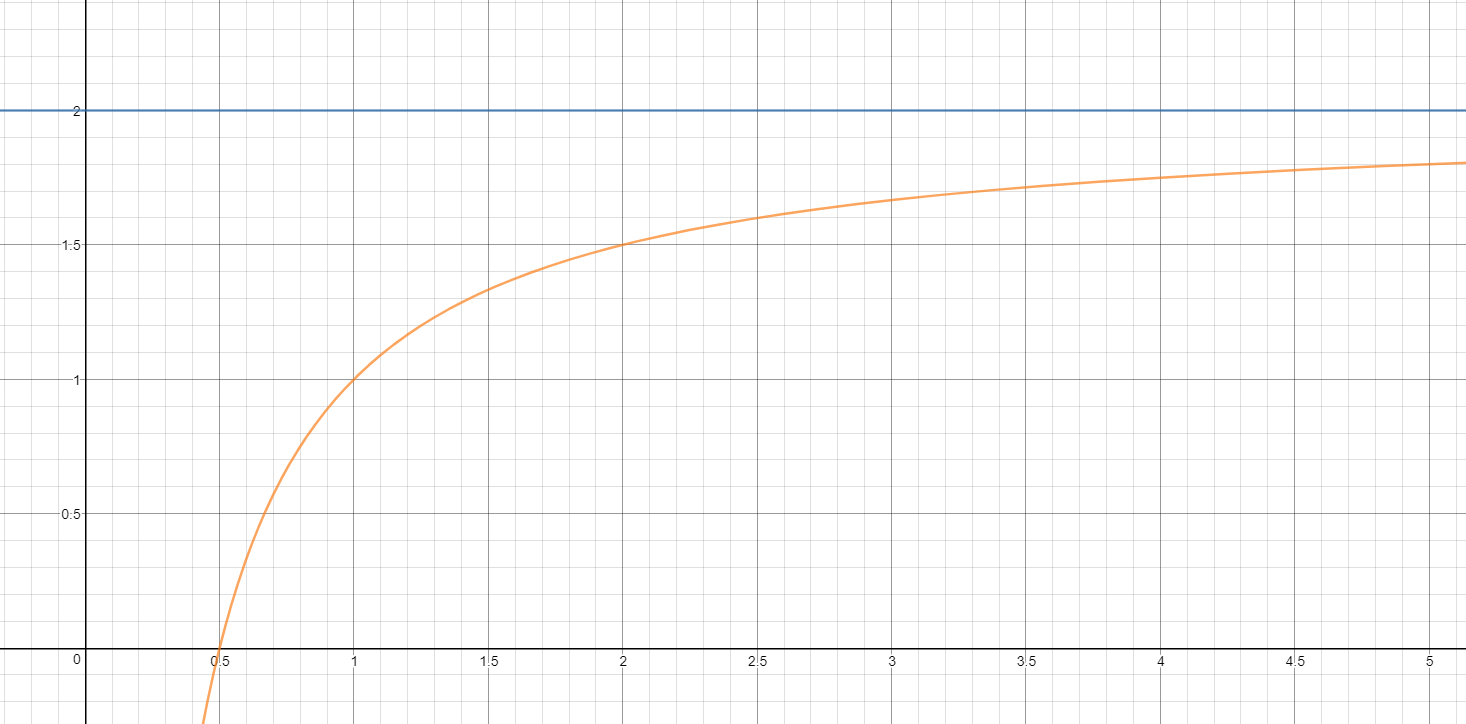
\includegraphics[scale=0.35]{graph.png}
		Even small improvements like these are celebrated results! \\~\ (i.e. Your money is being well spent)
	\end{frame}
	\begin{frame}{Motivation}
		\begin{itemize}[FAQ]
			\item<1-> Why are we trying to solve some problem like $k$-SAT?
			\item<1-> It's not even in poly time! Can I have my money back?
			\item<2-> Is there going to be a lot of talk about randomised algo?
		\end{itemize}
	\end{frame}
	\begin{frame}{Motivation}
		\begin{itemize}[FAQ]
			\item<1-> Why are we trying to solve some problem like $k$-SAT?
			\item<1-> It's not even in expected poly time! Can I have my money back?
			\item<1-> Is there going to be a lot of talk about randomised algo? Yes! 4 full pages. What a deal!
			\item<2-> "Derandomization". What is it and why are we 
						covering it?
		\end{itemize}
	\end{frame}
\section{Sch\"{o}ning's randomized algorithm}
	\begin{frame}{Intuition}
		\begin{block}{Intuition}
			If some instance of a $k$-SAT problem has some satisfying assignment $\alpha^*$, then given some assignment $\alpha$, there is some Hamming distance between $\alpha^*$ and $\alpha$ which counts the number of literals they disagree on. 
		\end{block}
		We will denote this as $\dist{\alpha^*}{\alpha}$.
		Idea: We can turn this into a random walk! Where each state of the Markov chain is the Hamming Distance from a given assignment $\alpha$ to the satisfying one $\alpha^*$. 	
	\end{frame}
	\begin{frame}{Algorithm description}
		\begin{algorithm}[H]
			\caption{$k$-SAT-Random-Walk}
			\DontPrintSemicolon
			\SetKwInOut{Input}{Input}\SetKwInOut{Output}{Output}
			\Input{$(F,\alpha,r)$}
			\Output{A satisfying assignment $\astar$ or NO if no $\astar$ are found}
			\BlankLine
			\For{steps = 1 to 3n}{
				\lIf{$\alpha$ satisfies $F$}{return $\alpha$}
				Choose an arbitrary clause $C$ not satified by $\alpha$\\
				Choose a literal in $C$ uniformly at random and flip its value in $\alpha$
			}
			\lIf{$\alpha$ satisfies $F$}{return $\alpha$}
			\hspace{7em}\lElse{return NO}
			\end{algorithm}
	\end{frame}
	\begin{frame}{Analysis}
		Just like in the case of 2-SAT, we would like to model the process as a random walk, where a state denotes the Hamming distance of the current assignment $\alpha$ from the actual satisfying assignment $\alpha^*$. \\~\
		
		At every step, the algorithm goes closer to $\alpha^*$ with probability of at least $\frac{1}{k}$, and with probability at most $1 - \frac{1}{k}$ it moves further away. \\~\
		
		Why? if there was a satisfying assignment, surely at least one of the literals has to be satisfied! And since there are $k$ literals, with probability at least $\frac{1}{k}$ we choose it. \\~\
	\end{frame}
	\begin{frame}{Analysis}
		\begin{theorem}
			(Proof Omitted) For an assignment $\alpha$ within some Hamming Distance $d$ away from a satisfying assignment $\alpha^*$, the algorithm finds $\alpha^*$ with probability $\geq (\frac{1}{k-1})^d$.
		\end{theorem}
		This actually follows from a detailed analysis of the previously mentioned random walk. 
		%% Maybe add more later on if possible.
	\end{frame}
	\begin{frame}{Analysis}
		Thus, the probability that the algorithm finds the assignment is:\\
		\begin{center}						
		\[
			\frac{1}{2}^n \cdot \mathlarger{‎‎\sum}_{j=0}^{n}\binom{n}{j}\frac{1}{k-1}^j = \big(\frac{1}{2}(1+\frac{1}{k-1})\big)^n
			= \big(\frac{k}{2(k-1)}\big)^n		
		\]		
		\end{center}
		amplifying this, the runtime of the algo should be:\\
		\begin{center}						
		\[
			\O\left(\Big(2\big(1-\frac{1}{k}\big)\Big)^n\right)
		\]		
		\end{center}
	\end{frame}
\section{Basic Derandomization with Local Search}
	\begin{frame}{Derandomizing the algorithm}
		\begin{enumerate}
		\item The choice of an initial assignment $\alpha$
		\item The random walk around the initial assignment.
		\end{enumerate}
	\end{frame}
	\begin{frame}{Idea}
		We can view the randomized algorithm as searching for the satisfying assignment within a certain radius.
		\begin{definition}[Hamming Ball]
			$B_r(\alpha)$ is called a Hamming Ball, which is the set of all assignments which have a Hamming Distance of at most $r$ from $\alpha$.\\
		\end{definition}
		\begin{definition}[Covering Code]
			A covering code of radius $r$ is a set of coordinates, which serve as the center for a Hamming Ball respectively, such that every coordinate in the space of every possible assignment is inside at least one Hamming Ball.\\
			Or if you prefer, every possible assignment is within $r$ Hamming distance of some element in the covering code.
		\end{definition}
	\end{frame}	
	\begin{frame}{Hamming Ball Properties}
	A Hamming Ball with a radius $r$ has a size of $\Sigma_{i=0}^{r}\binom{n}{i}$. 
	\end{frame}
	\begin{frame}{Hamming Ball Properties}
	For any $n \geq 1$ and $r$, there exits a covering code of size at most: 
	\begin{align*}
				\frac{n \cdot 2^n}{\Sigma_{i=0}^{r}\binom{n}{i}}
	\end{align*}
	We shall use a probabilistic argument:
	% Do the proof on a whiteboard.	
	\end{frame}
	\begin{frame}{Searching assignments from within distance $k$}
		\begin{algorithm}[H]
			\caption{$\PBS$-Recursion}
			\DontPrintSemicolon
			\SetKwInOut{Input}{Input}\SetKwInOut{Output}{Output}
			\Input{$(F,\alpha,r)$}
			\Output{A satisfying assignment $\astar$ or NO if no $\astar$ are found}
			\BlankLine
			\lIf{$\alpha$ satisfies $F$}{return $\alpha$}
			\hspace{7em}\lElseIf{r = 0}{return NO}
			Choose an arbitrary clause $C$ not satified by $\alpha$\\
			\ForEach{literal $l \in C$}{
			$\alpha'$ = $\PBS$-Recursion($F^{[l = 1]}, \alpha^{[l=1]},r-1)$\\
			\lIf {$\alpha'$ satisfies $F$}{Return $\alpha'$}
			}
			{return NO}
		\end{algorithm}
	\end{frame}
	\begin{frame}{Running time?}
		\begin{lemma}
			$\PBS \textnormal{-Recursion}$ solves $\PBS$ in $\O(k^r)$ time.
		\end{lemma}
		\begin{proof}
			The running time is straightforward. Each clause has at most $k$ literals and hence each node in the recursion tree has at most $k$ branches. The depth of the recursion three is at most $r$. Hence, there are at most $k^r$ leaves in the recursion tree. The overall runtime is $\O(k^r)$. \par 
		\end{proof}
	\end{frame}
	\begin{frame}{Putting it together}
		So now we derandomize the original algorithm. Recall that there were two things to derandomize. The initial choice of an assignment, and the random walk that starts from it. \\~\
		Elements from the code shall serve as the initial assignment, and the previously stated algorithm serves as our not-so-random walk.
	\end{frame}
	%% Use the whiteboard to explain, stuff like F[l=1] and so on. 
	\subsection{Derandomized Algorithm}
	\begin{frame}{Combining the two derandomizations}
	\begin{algorithm}[H]
	\caption{Deterministic $\SAT$}
	\DontPrintSemicolon
	\SetKwInOut{Input}{Input}\SetKwInOut{Output}{Output}
	\Input{A $\CNF$ formula $F$ with $n$ variables}
	\Output{A satisfying assignment $\astar$ or NO if no $\astar$ are found}
	\BlankLine
	Initialization: Compute covering code $\cc_{\rho n}$\\
	\ForEach{code $c \in \cc_{\rho n}$}{
		$\astar$ = $\PBS$-Recursion($F,c,\rho n$)\\
		\lIf{$\astar$ satisfies $F$}{return $\astar$}
	}
	{return NO}
\end{algorithm}
	\end{frame}
	\begin{frame}{Running time?}
		\begin{align*}
T(n,\rho,d) &= \O(2^{3n/d}+ 2^{(1-h(\rho))n}) + \O(2^{(1-h(\rho))n})\cdot \O(k^{\rho n}) \\~\
T(n,\rho,d) &=\O(2^{(1-h(\rho))n} \cdot k^{\rho n})\\~\
&= \O\Big(2^{(1+ \frac{1}{k+1}\log_2\frac{1}{k+1} + \frac{k}{k+1}\log_2\frac{k}{k+1})n} \cdot 2^{(\frac{1}{k+1} \log_2 k )n}\Big)\\~\
&= \O\Big(2^{(1 - \frac{1}{k+1}\log_2 (k+1) + \frac{k}{k+1}\log_2 k - \frac{k}{k+1}\log_2 (k+1) + \frac{1}{k+1} \log_2 k)n}\Big)\\~\
&= \O\Big(2^{(1 - \log_2 (k+1) + \log_2 k)n}\Big)\\~\
&= \O\Big(\big(2 \cdot \frac{k}{k+1}\big)^{n}\Big) = \O\Big(\big(2 - \frac{2}{k+1}\big)^n\Big)
		\end{align*} 
	\end{frame}
	\begin{frame}{Hmm}
		$\O\big((2 - \frac{2}{k+1})^n\big)$ seems a little too large. Turns out we can still improve it!
	\end{frame}
%% Zeyong's section onwards.
\section{Improving on the Derandomization}
	\begin{frame}{Aim}
	Overall running time: $\O\Big(\big(2(1-\frac{1}{k+1})\big)^n\Big)$\\
	Notice that the parameter $k$ comes from the running time of $\PBS$-Recursion, which is $\O(k^r)$.\\
	If we could improve it to $\O\big((k-1)^r\big)$, then we achieve the desired $\O\Big(\big(2(1-\frac{1}{k})\big)^n\Big)$ performance.
	\end{frame}
	\begin{frame}{Intuition}
	Observation 1: Whenever we fix an assignment for a variable, all clauses containing the variable would have one less literal to be considered. 
	\begin{example}
		Consider the following $3$-CNF formula:
	\begin{align*}
	&(x_1 \lor x_2 \lor x_3) \land (\bar{x_1} \lor x_4 \lor x_5)\\
	&\text{assigning }x_1 = 1\\
	&(1 \lor x_2 \lor x_3) \land (0 \lor x_4 \lor x_5)\\
	&(x_4 \lor x_5)
	\end{align*}
	\end{example}

	\end{frame}	
	\begin{frame}{Intuition}
	Observation 2: By flipping one variable at a time(or moving one step in the Markov chain), we are covering a Hamming Ball of radius $r$ with k Hamming Balls of radius $(r-1)$. \\~\
	What if we are more ambitious and change $t$ variables at a time? Can we do better by covering the BIG Hamming Ball with much smaller Hamming Balls? \\~\
	But how do we choose the $t$ variables? We need to modify our Covering Codes to help us.
	\end{frame}	
	\subsection{Extended Covering Codes}
	\begin{frame}{Introduction}
	We define a $k$-ary Covering Code to be analogous to the previous Covering Code but instead of from $\{0,1\}^t$, we define it to be from $\{1,...,k\}^t$ instead. \\~\
	Now each point has $t$ coordinates and each coordinate takes the value from $1$ to $k$. The notion of distance remains as the number of coordinates in which the two points disagree on.
	\begin{example}
		$w_1 = \{1, 1, 1\}$ $w_2 = \{1, 3, 3\}$ \\
		$\dist{w_1}{w_2} = 2$ as there are two different coordinates.
	\end{example}

	\end{frame}
	\begin{frame}{Size of the Covering Code}
	Let $V^k(r)$ denote the volume of a k-ary Hamming Ball of radius $r$. \\
	Number of points at whose distance is exactly $r$ from a particular point = $ {t \choose r}(k-1)^r$. Hence, $V^k(r) > {t \choose r}(k-1)^r$ \\
	By using a similar probabilistic argument as before, there exists a k-ary covering code $\cc_r^k$ such that 
	\begin{align*}
	|\cc^k_r| \leq \left \lceil \frac{t\ln(k)k^t}{{t \choose r}(k-1)^r} \right \rceil
	\end{align*}
	\end{frame}
	\begin{frame}{Size of the Covering Code}
	Lastly, by choosing $r = \frac{t}{k}$, and going through some algebra, we have the following bound:
	\begin{align*}
	|\cc^k_{{t/k}}| \leq \left \lceil \frac{t\ln(k)k^t}{{t \choose t/k}(k-1)^{t/k}} \right \rceil \leq \frac{t^2 k^t (k-1)^{(k-1)t/k}}{k^t(k-1)^{t/k}} \leq t^2(k-1)^{t-2t/k}
	\end{align*}
	\end{frame}
	\begin{frame}{How do we use k-ary Covering Code}
	 We apply a point $w \in \cc_r^k$ on a assignment $\alpha$ in the following manner: Let $H$ contains $t$ arbitrarily chosen clauses in $\alpha$. for the $i$th clause in $H$, let $p$ be the $i$th coordinate of $w$ and flip the value of the $p$th literal in the $i$th clause. We denote the new assignment as $\alpha[w]$.
	 \begin{example}			
	 	given $H = \{(x_1 \lor x_2 \lor x_3), (x_4 \lor x_5 \lor x_6)\}$ where all variables have value $0$ and $w = (2,3)$. Then we will have a new assignment by changing $x_2 = 1$ and $x_6 = 1$.
	 \end{example}
	\end{frame}
	\begin{frame}
	Assuming that all variables in $H$ are independent and all clauses are unsatisfied\\~\

	Suppose $w^*$ denotes the difference between assignment $\alpha$ and a satisfying assignment $\astar$ for the $t$ clauses in $H$. That is, we make $t$ correct moves towards $\astar$, $\dist{\alpha[w^*]}{\astar} \leq r - t$. \\
	We know $\exists w \in \cc_r^k$ such that $\dist{w}{w^*} \leq t/k$. Hence, the assignment $\alpha[w]$ makes at least $t - t/k$ correct moves and at most $t/k$ wrong moves.\\
	We have $\dist{\alpha[w]}{\astar} \leq r - (t - t/k) + t/k \leq r - (t-2t/k)$
\end{frame}
	\subsection{Improved Derandomized Algorithm}
	\begin{frame}{Algorithm}
	Before doing anything else, first compute a $k$-ary covering code $\cc_r^k$ of radius $\frac{t}{k}$, where $t$ is some constant. \\~\
	
	Upon the input of some $\CNF$ and a assignment $\alpha$, the algorithm greedily find the maximal independent set of unsatisfied clauses $G = \{C_1, C_2, ...,C_m\}$. \\
	\begin{enumerate}
		\item[1] Independent: any two clauses do not share any variables\\
		\item[2] Maximal: all other unsatisfied clauses (outside of $G$) share at least one variable with some $C_i$.
	\end{enumerate}
	Now we can break the problem instance into 2 cases: \\~\
	\end{frame}
	\begin{frame}
		\begin{enumerate}
			\item[1] $|G| \leq t$ : Enumerate all possible assignments for $G$ and run $\PBS$-Recursion on the new formula. \\~\
			Notice that all other unsatisfied clauses share at least one variable with $G$ which is now assigned a value. \\~\
			From observation 1, all unsatisfied clauses now have at most $k-1$ literals and the running time is $\O((k-1)^r)$.
		\end{enumerate}
	\end{frame}	
	\begin{frame}
		\begin{enumerate}
			\item[2] $|G| > t$: Arbitrarily choose a set $H \subseteq G$ such that $H$ is of size $t$. Now apply the k-ary covering code in the following manner: for each point $w \in \cc_r^k$, apply $w$ on $H$ and we have a new assignment $\alpha[w]$. Then recurse with $r' = r - (t - 2t/k)$\\~\
		\end{enumerate}
	\end{frame}	
	\begin{frame}
		Lastly, let us look at the running time. Let $\delta = t - 2t/k$. The recursion tree has $|\cc_r^k|$ branches and $r$ decreases by $\delta$ in each step. Hence, the height is ${r/\delta}$. The number of leaves is at most
		\begin{align*}
		|\mathcal{C}_r^k|^{r/\delta} &\leq (t^{2}(k-1)^{\delta})^{r/\delta}\\
		&= \big((k-1)t^{2/\delta}\big)^{r}
		\end{align*}
		Note that $t$ is independent of the input size and the running time is thus $\O\big((k-1)^r\big)$.
	\end{frame}

\subsection{Take Away}
\begin{frame}
	3 key ideas:
	\begin{enumerate}
		\item[1] Randomization can give intuition for deterministic search
	\end{enumerate}
\end{frame}
	\begin{frame}
Questions?
\end{frame}
\end{document}